%%
%% This is file `sample-manuscript.tex',
%% generated with the docstrip utility.
%%
%% The original source files were:
%%
%% samples.dtx  (with options: `manuscript')
%% 
%% IMPORTANT NOTICE:
%% 
%% For the copyright see the source file.
%% 
%% Any modified versions of this file must be renamed
%% with new filenames distinct from sample-manuscript.tex.
%% 
%% For distribution of the original source see the terms
%% for copying and modification in the file samples.dtx.
%% 
%% This generated file may be distributed as long as the
%% original source files, as listed above, are part of the
%% same distribution. (The sources need not necessarily be
%% in the same archive or directory.)
%%
%% The first command in your LaTeX source must be the \documentclass command.
\documentclass[manuscript,screen,review]{acmart}

%%
%% \BibTeX command to typeset BibTeX logo in the docs
\AtBeginDocument{%
  \providecommand\BibTeX{{%
    \normalfont B\kern-0.5em{\scshape i\kern-0.25em b}\kern-0.8em\TeX}}}

% %% Rights management information.  This information is sent to you
% %% when you complete the rights form.  These commands have SAMPLE
% %% values in them; it is your responsibility as an author to replace
% %% the commands and values with those provided to you when you
% %% complete the rights form.
% \setcopyright{acmcopyright}
% \copyrightyear{2018}
% \acmYear{2018}
% \acmDOI{10.1145/1122445.1122456}

% %% These commands are for a PROCEEDINGS abstract or paper.
% \acmConference[Woodstock '18]{Woodstock '18: ACM Symposium on Neural
%   Gaze Detection}{June 03--05, 2018}{Woodstock, NY}
% \acmBooktitle{Woodstock '18: ACM Symposium on Neural Gaze Detection,
%   June 03--05, 2018, Woodstock, NY}
% \acmPrice{15.00}
% \acmISBN{978-1-4503-XXXX-X/18/06}


%%
%% Submission ID.
%% Use this when submitting an article to a sponsored event. You'll
%% receive a unique submission ID from the organizers
%% of the event, and this ID should be used as the parameter to this command.
%%\acmSubmissionID{123-A56-BU3}

%%
%% The majority of ACM publications use numbered citations and
%% references.  The command \citestyle{authoryear} switches to the
%% "author year" style.
%%
%% If you are preparing content for an event
%% sponsored by ACM SIGGRAPH, you must use the "author year" style of
%% citations and references.
%% Uncommenting
%% the next command will enable that style.
%%\citestyle{acmauthoryear}
\usepackage{hyperref}
%%
%% end of the preamble, start of the body of the document source.
\begin{document}

%%
%% The "title" command has an optional parameter,
%% allowing the author to define a "short title" to be used in page headers.
\title{Dynamic Task Scheduling with Unsupervised Self Organizing Map}

%%
%% The "author" command and its associated commands are used to define
%% the authors and their affiliations.
%% Of note is the shared affiliation of the first two authors, and the
%% "authornote" and "authornotemark" commands
%% used to denote shared contribution to the research.

\author{Zhimo Zhou}
\authornote{Both authors contributed equally to this research.}
\email{zzhou17@uoguelph.ca}
% \orcid{1234-5678-9012}
\affiliation{%
  \institution{Universe of Guelph}
  \streetaddress{500 Stone Rd, E}
  \city{Guelph}
  \state{Ontario}
  \country{Canada}
  \postcode{N2L 3G1}
}  
\author{Uday Singh}
\authornote{Both authors contributed equally to this research.}
\email{usingh03@uoguelph.ca}
% \orcid{1234-5678-9012}
\affiliation{%
  \institution{Universe of Guelph}
  \streetaddress{500 Stone Rd, E}
  \city{Guelph}
  \state{Ontario}
  \country{Canada}
  \postcode{N2L 3G1}
}
\author{Yaowen Mei}
\authornote{Both authors contributed equally to this research.}
\email{ywmei@uoguelph.ca}
% \orcid{1234-5678-9012}
\affiliation{%
  \institution{Universe of Guelph}
  \streetaddress{500 Stone Rd, E}
  \city{Guelph}
  \state{Ontario}
  \country{Canada}
  \postcode{N2L 3G1}
}
%%
%% By default, the full list of authors will be used in the page
%% headers. Often, this list is too long, and will overlap
%% other information printed in the page headers. This command allows
%% the author to define a more concise list
%% of authors' names for this purpose.
% \renewcommand{\shortauthors}{Trovato and Tobin, et al.}

%%
%% The abstract is a short summary of the work to be presented in the
%% article.
\begin{abstract}
Some Abstract I will add later
\end{abstract}

%%
%% The code below is generated by the tool at http://dl.acm.org/ccs.cfm.
%% Please copy and paste the code instead of the example below.
%%
\begin{CCSXML}
<ccs2012>
   <concept>
       <concept_id>10003456.10003457.10003521.10003524</concept_id>
       <concept_desc>Social and professional topics~History of software</concept_desc>
       <concept_significance>500</concept_significance>
       </concept>
   <concept>
       <concept_id>10010520.10010521</concept_id>
       <concept_desc>Computer systems organization~Architectures</concept_desc>
       <concept_significance>500</concept_significance>
       </concept>
 </ccs2012>
\end{CCSXML}

\ccsdesc[500]{Social and professional topics~History of software}
\ccsdesc[500]{Computer systems organization~Architectures}

%%
%% Keywords. The author(s) should pick words that accurately describe
%% the work being presented. Separate the keywords with commas.
\keywords{ Android Studio, Eclipse, Apache Maven, Gradle, Software Architecture}
%%
%% This command processes the author and affiliation and title
%% information and builds the first part of the formatted document.
\maketitle
\section{Introduction}
Self-Organizing Map (SOM), also know as Kohonen map, is a topological preserving map that can map a higher dimensional space to a lower dimensional space. Along this process, information will be compressed; while, the key parameters in terms of "topological and metric relationships"\cite{Kohonen1998} will be retained. 
\\
There are two steps involved in forming a self-organizing map from a raw input data-set\cite{hebbian2007}, respectively to be 1) \textbf{competition} and 2) \textbf{cooperation}. When a set of data is feed into the system sequentially with random shuffle, for each input data point, \textbf{competition} will take place first and, based on a pre-defined cost function, one of the neurons on the output layer with the minimal cost will be selected as a winner; Following the competition, the  \textbf{cooperation} will then take place. Based on a neighborhood function, the winner together with it's neighbor neurons will proceed the learning; while, the neurons outside of the winner's neighbor zone will gain no learning. The purpose of the cooperation step is to increase the like-hood that if a similar input pattern present again, the same group of neurons will become the winner with a higher possibility. Iterate with this strategy on the input data-set over a suitable period, without supervising (providing error to the system), the output layer will simultaneously form a map that contains the similar topological structure as the input data. 



\begin{figure}[h]
  \centering
  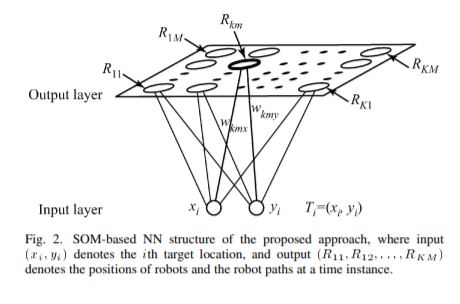
\includegraphics[width=8cm]{Picture/AnminPic.JPG}
  \caption{The illustration of the intermediate step to map K inputs (Robots) to M outputs (Targets)\cite{zhu2006neural}. At a time instance, $i$, K neurons out of these $K*M$ possibilities will be selected as the winner. [\textcolor{red}{I do not really understand this!!!, should we have K winner as we only have K inputs or M winner as each neuron should have same possibility to win???}] }
  \Description{More People are using Maven as build tool than Gradle}
\end{figure}


\section{Model and Method}
\begin{itemize}
    \item 1D model of K robots and M Targets
    \item 2D model of K robots and M Targets
    \item KD model of K robots and M targets
\end{itemize}



% \section{Objectives and Milestones}
\subsection{List of Objectives}
\begin{enumerate}
    \item Experience both Gradle and Maven
    \item Compare the different features provided by Gradle and Maven
    \item Compare the efficiency between Gradle and Maven when building an Android Project
    \item Do the SWOT (Strengths, Weaknesses, Opportunities and Threats) analysis for both Gradle and Maven, and find out which one is better.
\end{enumerate}


\subsection{The Milestones}
\begin{enumerate}
    \item Develop an Android App with Android Studio + Gradle, then write the same Android app with Eclipse + Maven to get familiar with Maven
    \item Based on the experience in (1), write 2 pages report to discuss the different features provided by Maven and Gradle (I have registered for the "Introduction to Gradle Build Tool" workshop \url{https://gradle.com/training/introduction-to-gradle-july/?time=1626739200} on July 20-21 from Gradle's website so that I can have a better understanding about different features provided by Gradle )
    \item Learn how to "build cache" for both Maven and Gradle, and compare the efficiency between Gradle and Maven. (I have also registered for the "Introduction to Developer Productivity Engineering" workshop \url{https://gradle.com/training/dpe-workshop/?time=1623628800} on June 14 so that I can understand how exactly Gradle and Maven are handling the building ache task).
    \item Finish this article by analysing the difference in design pattern between Maven and Gradle, and make a conclusion which build tool has better future.
\end{enumerate}


%%
%% The acknowledgments section is defined using the "acks" environment
%% (and NOT an unnumbered section). This ensures the proper
%% identification of the section in the article metadata, and the
%% consistent spelling of the heading.
% \begin{acks}
% To Robert, for the bagels and explaining CMYK and color spaces.
% \end{acks}

%%
%% The next two lines define the bibliography style to be used, and
%% the bibliography file.
\bibliographystyle{ACM-Reference-Format}
\bibliography{sample-base}


\end{document}
\endinput
%%
%% End of file `sample-manuscript.tex'.
